\documentclass{beamer}
\mode<presentation>
\usetheme{CambridgeUS}
\usepackage[russian]{babel}
\usepackage[utf8]{inputenc}
\usepackage[T2A]{fontenc}
\usepackage{sansmathaccent}

\usepackage{verbatim}
\usepackage{alltt}

\pdfmapfile{+sansmathaccent.map}
\title[Software Design]{Основы объектно-ориентированного программирования}
\author{Наумов Д.А., доц. каф. КТ}
\date[05.10.2019] {Основы программной инженерии, 2020}

\begin{document}

%ТИТУЛЬНЫЙ СЛАЙД
\begin{frame}
  \titlepage
\end{frame}
  
%СОДЕРЖАНИЕ ЛЕКЦИИ
\begin{frame}
  \frametitle{Содержание лекции}
  \tableofcontents  
\end{frame}
  
\section{Элементы объектной модели}
\begin{frame}
Объектную модель составляют четыре главных элемента:
\begin{itemize}
\item абстрагирование (abstraction) - выделение существенных характеристик некоторого объекта, отличающие его от всех других видов объектов;
\item инкапсуляция (encapsulation) - отделение друг от друга элементов объекта, определяющих его устройство и поведение; представление системы в виде совокупности обособленных сегментов (модульность);
\item иерархия (hierarchy) - упорядочение абстракций, средство классификации объектов, систематизация связей между объектами.
\item полиморфизм (polymorphism) - механизм, позволяющий заменять поведение объектов производных классов.
\end{itemize}
\end{frame}

\begin{frame}{Абстракция}
\begin{block}{Абстракция}
выделяет существенные характеристики некоторого объекта, отличающие его от всех других видов объектов и, таким образом, четко определяет его концептуальные границы с точки зрения наблюдателя.
\end{block}
Два вида абстракций в ООП:
\begin{itemize}
\item \textbf{тип данных объектной природы (класс)}— определяемое программистом
расширение исходных типов языка;
\item \textbf{экземпляр класса (объект)} — переменная класса. Объект обладает состоянием, поведением и идентичностью.
\end{itemize}
Состояние объекта:
\begin{itemize}
\item характеризуется набором его свойств (атрибутов) и текущими значениями каждого из этих свойств;
\item результат его поведения.
\end{itemize}
\end{frame}

\begin{frame}{Инкапсуляция}
Инкапсуляция предполагает возможность ограничения доступа к данным класса из других классов (python: namespaces). 
\begin{itemize}
\item это позволяет упростить интерфейс класса, показав наиболее существенные для внешнего пользователя данные и методы;
\item скрытие реализации обеспечивает возможность внесения изменений в реализацию класса без изменения других классов.
\end{itemize}
\end{frame}

\begin{frame}{Типы структурных иерархий}
Иерархическая декомпозиция и иерархическая организация ПО образуют один из основных систематических методов преодоления сложности программного обеспечения.
\begin{itemize}
\item cтруктурная иерархия "is-part-of" (агрегирование как разновидность ассоциации)
\item Структурные иерархии "is-а" и "is-like-a"
\end{itemize}
\end{frame}

\begin{frame}
\begin{block}{Обобщение}
означает, что объекты классапотомка могут использоваться везде, где допустимы объекты родительского класса. 
\end{block}
\begin{itemize}
\item Создавая базовый тип (базовый класс), программист выражает наиболее общие идеи относительно объектов, из которых конструируется программа.
\item В производных классах программист уточняет различия в реализации конструкций базового класса.
\item Производный класс полностью дублирует интерфейс базового класса, т. е. дублирует наблюдаемое поведение объекта базового класса. 
\item Поведение объекта производного класса может отличаться от поведения объекта базового класса.
\end{itemize}
\end{frame}

\begin{frame}{Полиморфизм}
Поведение объектов, на которых вызываются видоизмененные методы, интерфейс к которым заявлен в базовом классе, называют \textbf{полиморфным}, а механизм, обеспечивающий такое поведение, называют \textbf{полиморфизмом}.

Мы имеем возможность:
\begin{itemize}
\item работая с объектами разных типов, представляющих различные абстракции, мы можем использовать методы, которые имеют одинаковый интерфейс, что, в конечном счете, упрощает и реализацию программы, и ее восприятие;
\item разрабатывать общие процедуры обработки объектов.
\end{itemize}
\end{frame}

\section{Структура и организация определения класса}
\begin{frame}
\textbf{Задача классов} - предоставить программисту инструмент для создания новых типов данных с тем, чтобы их можно было без ограничений использовать в программе наряду со встроенными типами.

\textbf{Тип данных} является вопложением некоторой концепции (пример: целые числа), которое определяется рядом характеристик:
\begin{itemize}
\item областью применения типа;
\item способом представления типа в памяти;
\item множеством операций, разрешенных для этого типа;
\item множеством совместимых типов.
\end{itemize}
Новые типы создаются для воплощения концепций, которые \textit{не выражаются непосредственно} (или адекватно) встроенными типами.
\end{frame}

\begin{frame}{Класс - элемент абстракции}
\begin{itemize}
\item Определяя класс, мы создаем программную сущность, позволяющую выделить существенные характеристики некоторого объекта, отличающие его от других видов объектов.
\item Мы отделяем друг от друга элементы объекта, определяющие его устройство (\textbf{элементы-данные}), от элементов, определяющих его поведение (\textbf{элементы-действия}).
\item Данные, объявленные внутри определения класса, могут, в частности, быть п\textbf{еременными-членами класса} и \textbf{константами-членами класса}. 
\item Функции, объявленные внутри определения класса, называются \textbf{функциями-членами класса}, или \textbf{методами} класса.
\end{itemize}
\end{frame}

\begin{frame}[t]{Диаграмма классов}
\begin{figure}[h]
\centering
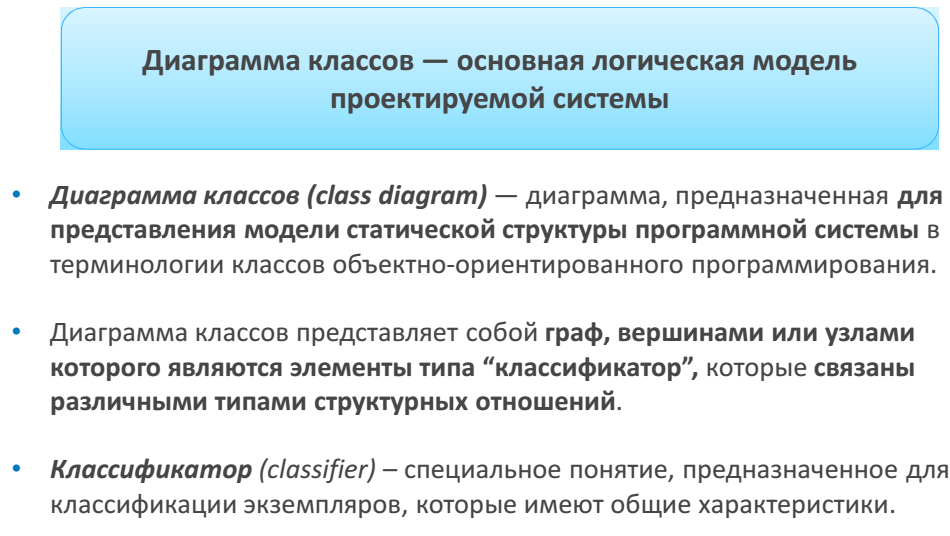
\includegraphics[scale=0.45]{images/lec03-pic16.png}
\end{figure}
\end{frame}

\begin{frame}[t]{Диаграмма классов}
\begin{figure}[h]
\centering
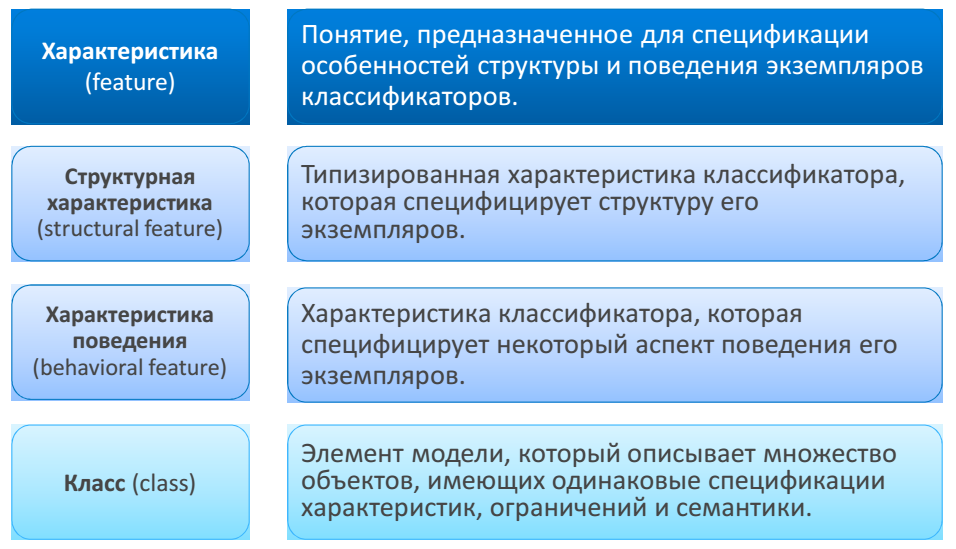
\includegraphics[scale=0.45]{images/lec03-pic17.png}
\end{figure}
\end{frame}

\begin{frame}[t]{Диаграмма классов}
\begin{figure}[h]
\centering
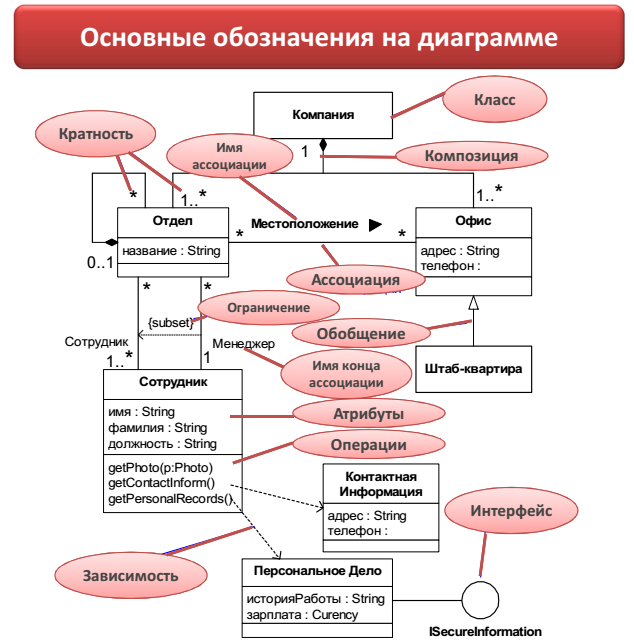
\includegraphics[scale=0.45]{images/lec03-pic18.png}
\end{figure}
\end{frame}

\begin{frame}[t]{Диаграмма классов}
\begin{figure}[h]
\centering
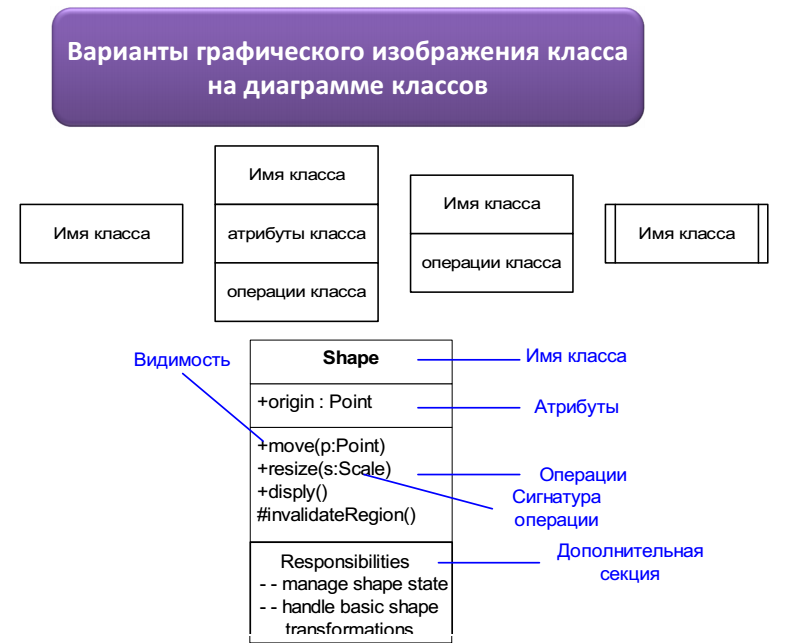
\includegraphics[scale=0.45]{images/lec03-pic19.png}
\end{figure}
\end{frame}

\begin{frame}[t]{Диаграмма классов}
\begin{figure}[h]
\centering
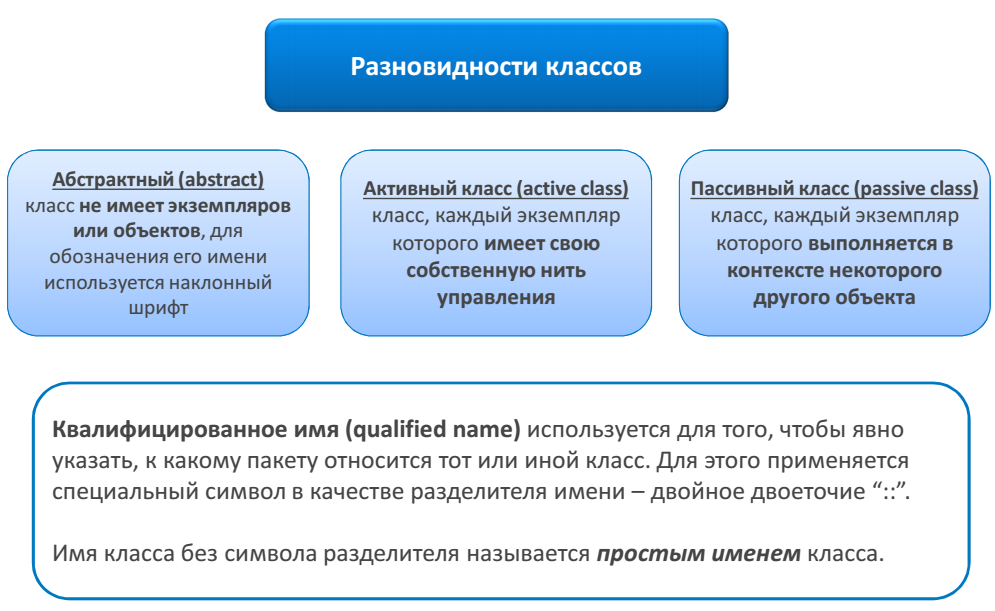
\includegraphics[scale=0.45]{images/lec03-pic20.png}
\end{figure}
\end{frame}

\begin{frame}[t]{Диаграмма классов}
\begin{figure}[h]
\centering
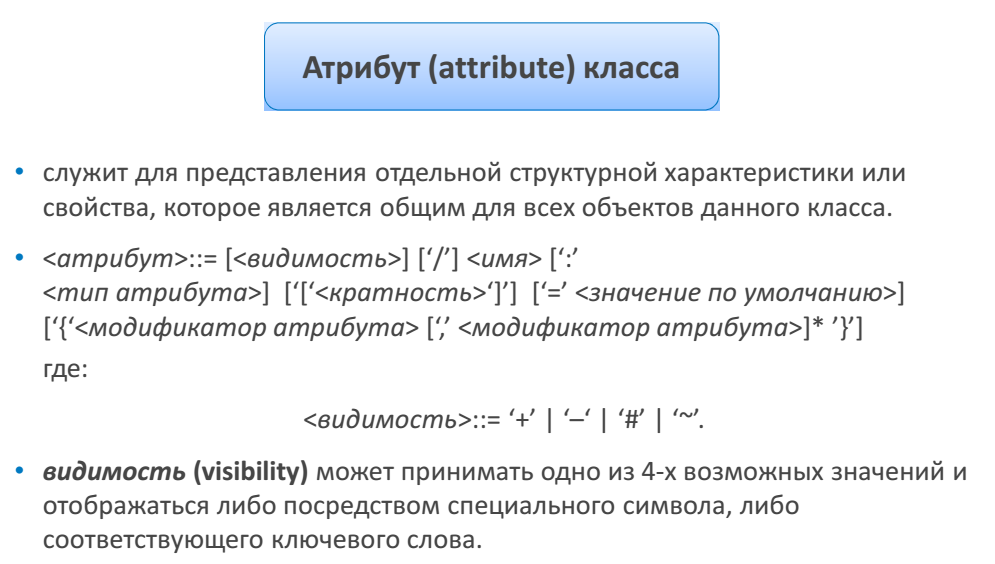
\includegraphics[scale=0.45]{images/lec03-pic21.png}
\end{figure}
\end{frame}

\begin{frame}[t]{Диаграмма классов}
\begin{figure}[h]
\centering
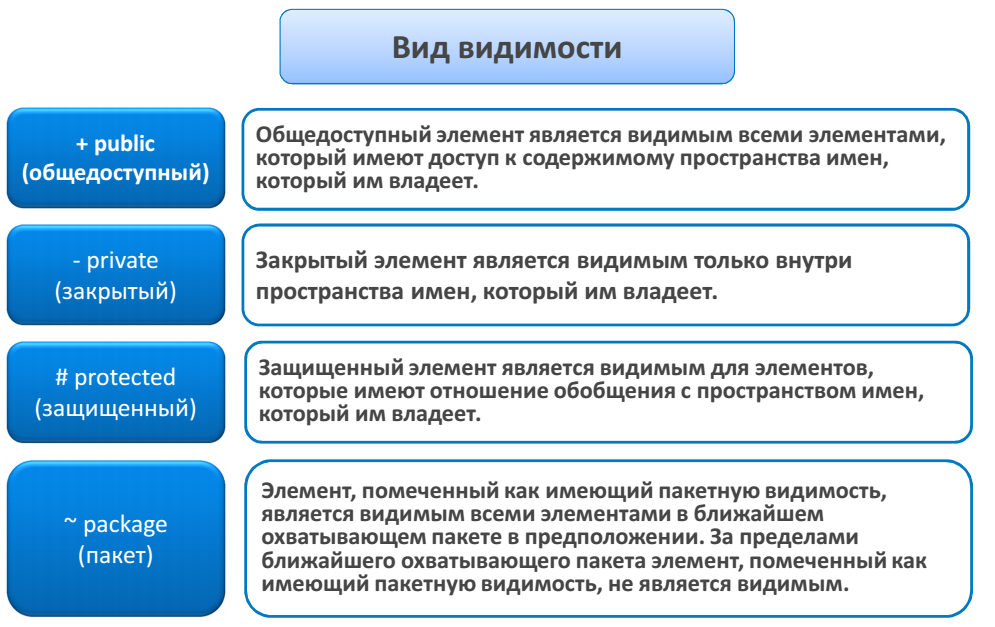
\includegraphics[scale=0.45]{images/lec03-pic22.png}
\end{figure}
\end{frame}

\begin{frame}[t]{Диаграмма классов}
\begin{figure}[h]
\centering
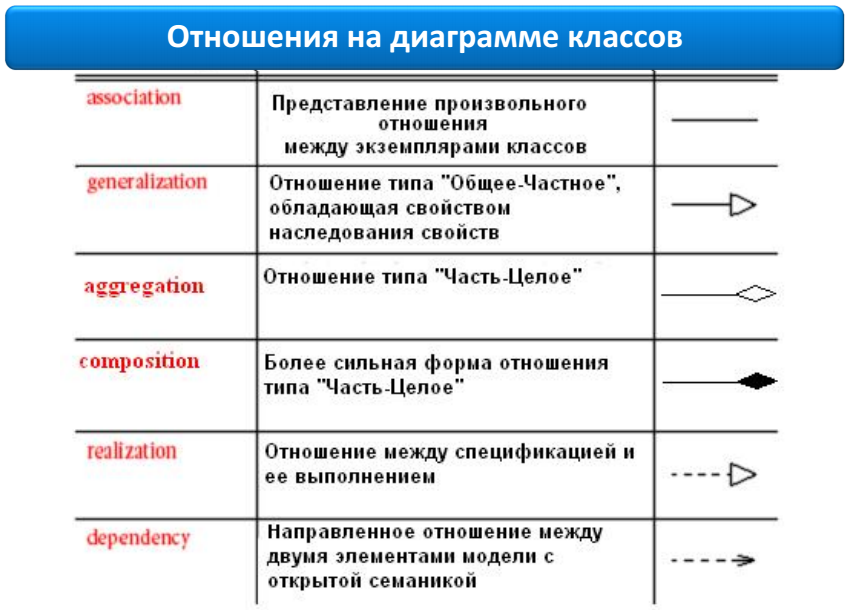
\includegraphics[scale=0.45]{images/lec03-pic23.png}
\end{figure}
\end{frame}

\begin{frame}[t]{Диаграмма классов}
\begin{figure}[h]
\centering
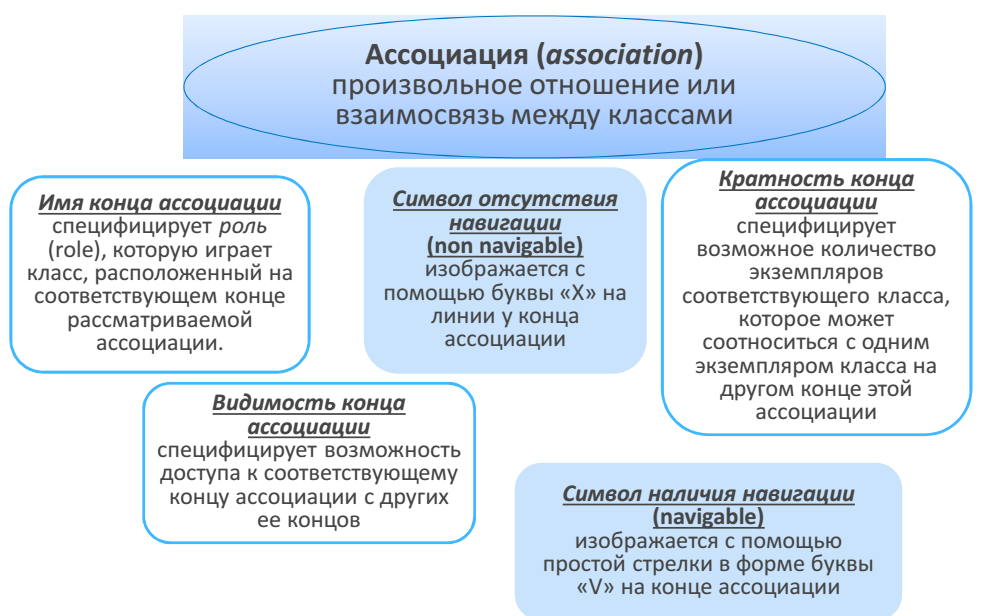
\includegraphics[scale=0.45]{images/lec03-pic24.png}
\end{figure}
\end{frame}

\begin{frame}{Отношения классов}
\begin{itemize}
\item \textbf{Отношение обобщения} (generalization) описывает отношение между общей
сущностью и ее конкретным воплощением (один класс является специализацией другого класса);
\item \textbf{Отношение ассоциации} (association) описывает структурное отношение,
показывающее, что объекты одного типа некоторым образом связаны
с объектами другого типа (находятся в отношении типа "часть/целое").
\item \textbf{Отношение зависимости} (dependency) описывает отношение использования, при котором изменение в спецификации одного класса может повлиять на класс, его использующий (объекты некоторого класса передаются в качестве аргументов функциям-членам другого класса).
\item \textbf{Отношение реализации} (realization) - семантическое отношение, при котором класс гарантирует выполнение контракта, определяемого некоторым интерфейсом.
\end{itemize}
\end{frame}

\begin{frame}{Отношение обощения}
\begin{figure}[h]
\centering
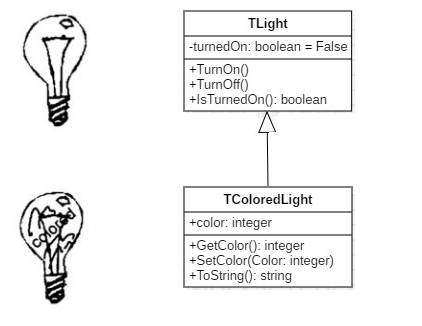
\includegraphics[scale=0.75]{images/lec04-pic10.png}
\end{figure}
\end{frame}

\begin{frame}{Отношение ассоциации}
\begin{figure}[h]
\centering
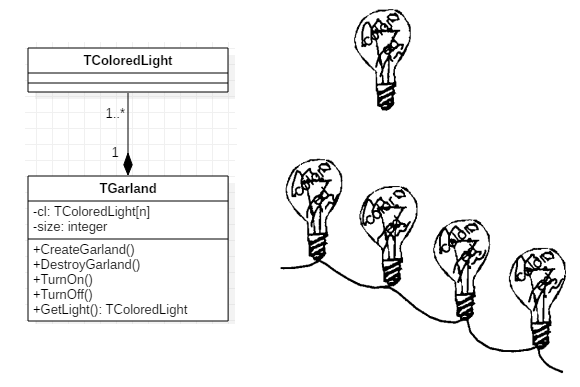
\includegraphics[scale=0.75]{images/lec04-pic14.png}
\end{figure}
\end{frame}

\begin{frame}{Отношение зависимости}
\begin{block}{Отношение зависимости}
является таким типом отношений между классами, когда изменение в спецификации или реализации одного класса влияет на спецификацию или реализацию другого класса.
\end{block}
\begin{figure}[h]
\centering
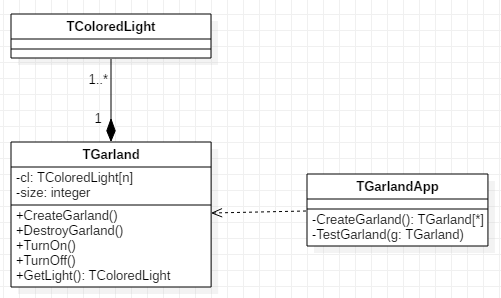
\includegraphics[scale=0.6]{images/lec04-pic18.png}
\end{figure}
\end{frame}

\begin{frame}{Отношение реализации}
\begin{block}{Отношение реализации}
используется для определения отношения между интерфейсом и классом, реализующим интерфейс.
\end{block}
Интерфейс определяет набор элементов (как правило, действий), характерных для объектов, обладающих определенными свойствами.
\begin{figure}[h]
\centering
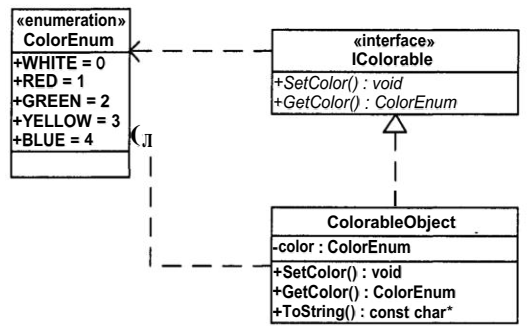
\includegraphics[scale=0.5]{images/lec04-pic19.png}
\end{figure}
\end{frame}

\begin{frame}
\begin{figure}[h]
\centering
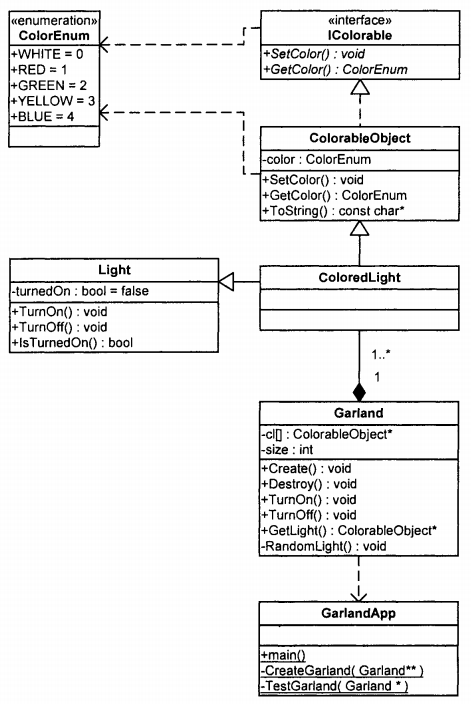
\includegraphics[scale=0.45]{images/lec04-pic21.png}
\end{figure}
\end{frame}

\end{document}
